% =====================================================================
% 附录 AU：测量、不确定度与数据分析 —— 从原始信号到误差棒（注明出处）
% ---------------------------------------------------------------------
% 数值唯一来源：tmp/appAU_calc.py（只 print，不写文件；输出 tmp/appAU_calc.txt）
%   工作点沿用全书 D1：n_e0 = 1e20 m^-3、T_e = 9.194 keV、B = 5.3 T、a = 2.0 m、R = 6.2 m
%   例：汤姆孙散射每点 200 个光子、单点统计误差 5%（相对）、B 类系统误差 2%（均匀分布）
%   跨附录对照：附录 AQ 的相位分辨 sigma_phi = 0.000361482 rad
% 单位口径：不确定度一律写成「相对百分数 + 绝对量」两份；角度用度，频率用 Hz，
%   长度用 m 与 nm 并标出换算；卡方与自由度无量纲。
% 与相邻附录的分工：
%   附录 Q 讲诊断原理（探针、光谱），附录 AQ/AN/AS/AH 讲各自的信号链，
%   本附录只讲「这些信号怎样变成一根误差棒」：合成、传播、拟合、区间、设计、陷阱。
%   附录 I 有「测量与不确定度」一节，讲的是学习动作；本附录给可直接代入的公式与数字。
% 版权口径：公式与量级口径取自公开发表的经典教材与标准（见 AU.8 来源表），
%   只保留本书诊断场景需要的部分，不复制原书的推导、代码与图表。
% =====================================================================
\section{从信号到误差棒：一根棒子里的三笔账}
\label{sec:app-au-budget}

前面每一个诊断附录最后都会落到一个数上：密度多少、温度多少、杂质份额多少。但一个数
如果没有误差棒，它就不是结论，只是一次读数。本附录要回答的问题是：从原始信号到这个
数，误差是怎样一笔一笔加上去的，又该怎样把它们写成读者能复核的形式。

先看一个具体例子。汤姆孙散射测电子温度：每个空间点用 200 个光子做一次统计，
单点统计误差（相对）取 $5\%$；另一条腿来自标定与几何，属于系统项，取 $2\%$。
统计项与系统项互相独立时，合成不确定度按方和根相加：
\begin{equation}
u_\mathrm{c}=\sqrt{u_\mathrm{stat}^2+u_\mathrm{sys}^2}
=\sqrt{0.05^2+0.02^2}=0.0538516,
\label{eq:app-au-uc}
\end{equation}
即 $u_\mathrm{c}=5.38516\%$。乘以覆盖因子 $k=2$（约 $95\%$ 置信）得到扩展不确定度
\begin{equation}
U=k\,u_\mathrm{c}=2\times0.0538516=0.107703,
\label{eq:app-au-U}
\end{equation}
也就是 $U=10.77033\%$。折合成绝对量：$n_\mathrm{e}=10^{20}\pm5.38516\times10^{18}\ \mathrm{m^{-3}}$。

一个数该不该接受，要先说清判据。若判据是 $15\%$，这个测量是合格的；若判据是 $10\%$，
它超了 $0.77033$ 个百分点，必须改设计。改法不是「多测几次」（系统项不随次数变小），
而是把统计项压下去：要求 $U\le5\%$ 即 $u_\mathrm{c}\le0.025$，在 $u_\mathrm{sys}=0.02$
不动的前提下，统计项要降到 $0.015$，也就是光子数乘以 $11.1111$ 倍——
从 $200$ 个加到 $2223$ 个。这就是一根误差棒背后的第一笔账。

\begin{table}[htbp]
\centering
\small
\caption{一根误差棒里的三笔账（例：单点统计 $5\%$、系统 $2\%$）}
\label{tab:app-au-budget}
\begin{tabular}{p{3.2cm}p{3.0cm}p{4.4cm}p{4.2cm}}
\hline
项目 & 来源 & 处理方式 & 例（相对） \\
\hline
统计项 $u_\mathrm{stat}$ & 有限计数、有限光子数、有限采样 & 随测量次数 $n$ 按 $1/\sqrt{n}$ 变小 & $5\%$ \\
系统项 $u_\mathrm{sys}$ & 标定、几何、模型近似、仪器刻度 & 不随重复次数变小，按 B 类处理 & $2\%$ \\
合成 $u_\mathrm{c}$ & 以上两项独立时的方和根 & $u_\mathrm{c}=\sqrt{u_\mathrm{stat}^2+u_\mathrm{sys}^2}$ & $5.38516\%$ \\
扩展 $U$ & 覆盖因子 $k$（本附录统一取 $2$） & $U=k\,u_\mathrm{c}$ & $10.77033\%$ \\
\hline
\end{tabular}
\end{table}

\begin{tip}{误差棒不是装饰，它是结论的一部分}{tip-app-au-budget}
一个数只有写成「值 $\pm$ 不确定度」并且说明覆盖因子，才是可以复核的结论；
只写中心值的表格，在物理上是不可用的。
\end{tip}

本节凡标出数字的量都由 \texttt{tmp/appAU\_calc.py} 复算。

\textbf{出处：}JCGM 100:2008《测量不确定度表示指南》（GUM）第 4--5 章给出合成与扩展
不确定度的国际口径；Taylor, \emph{An Introduction to Error Analysis}（2nd ed., 1997）
第 3 章给出本书采用的入门写法。

\begin{figure}[htbp]
\centering
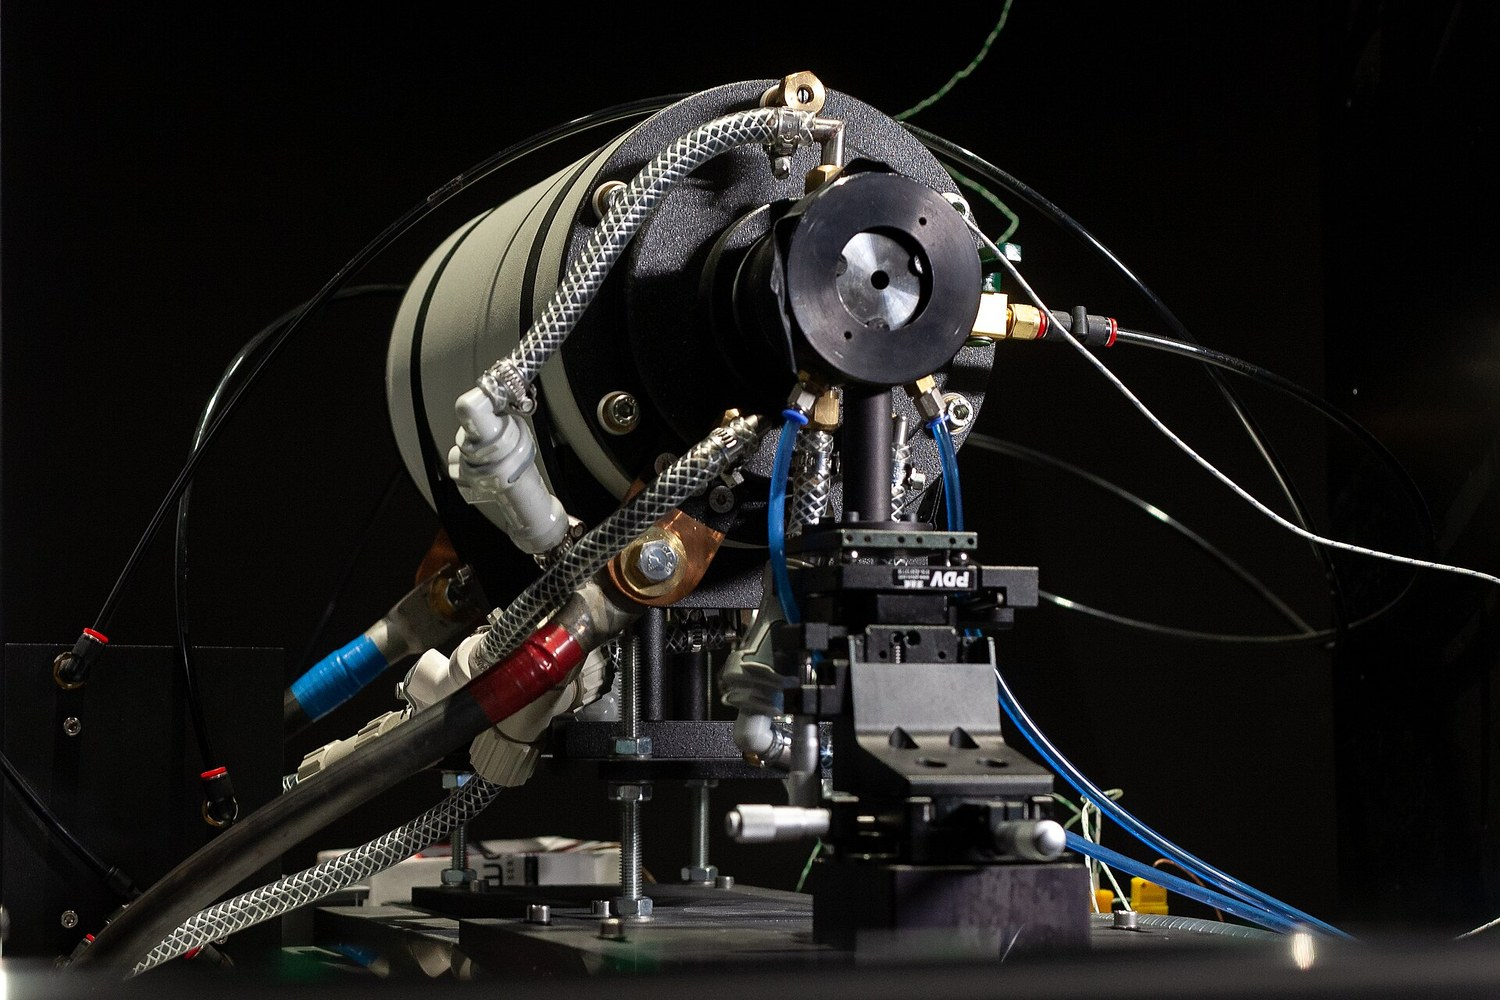
\includegraphics[width=0.78\textwidth]{../figures/blackbody_carlo.jpg}
\caption{黑体辐射源：误差棒的另一端是标准。任何一条误差棒都要有溯源链：黑体辐射源给出已知温度的基准，探测器读数才谈得上不确定度。本节把 A 类统计与 B 类系统合成成一条误差棒，而 B 类里的每一项，追到底都是这样的标准器。}
\label{fig:photo-appau2}
\figsource{Luminforum，CC BY 4.0（Wikimedia Commons）}
\end{figure}

\section{两条腿：A 类统计、B 类系统与合成}
\label{sec:app-au-class}

上一节把两笔账分开了，但「A 类」「B 类」的划分标准常被误解。标准不是「大小」，
而是\textbf{能不能靠多测几次变小}：A 类来自重复测量的散布，可以用统计方法估计，也随
$\sqrt{n}$ 下降；B 类来自刻度、标定、模型和手册数据，重复测量不会让它变小，只能用
已有信息给出一个区间。

A 类的标准写法是
\begin{equation}
u_\mathrm{A}=\frac{s}{\sqrt{n}},
\label{eq:app-au-uA}
\end{equation}
其中 $s$ 是 $n$ 次重复测量的样本标准差。取 $s=0.05$、$n=20$，得
$u_\mathrm{A}=0.0111803$，即 $1.11803\%$。注意这里除以了 $\sqrt{20}$：
把「单次测量的散布」变成「均值的散布」，这一步最容易被漏掉。

B 类在只有一个区间（比如「$\pm2\%$」）而没有分布信息时，按均匀分布处理：
\begin{equation}
u_\mathrm{B}=\frac{a}{\sqrt{3}},
\label{eq:app-au-uB}
\end{equation}
取 $a=0.02$ 得 $u_\mathrm{B}=0.011547$，即 $1.15470\%$。两条腿合成
$u_\mathrm{c}=0.0160728$，即 $1.60728\%$；取 $k=2$ 得 $U=3.21455\%$。
对照上一节可以看到一个容易被忽略的事实：\textbf{同一个 $5\%$ 的单次散布，一旦变成
$20$ 次测量的均值，对合成的贡献就从 $5\%$ 掉到 $1.11803\%$}。

严格说，$k=2$ 只在大样本下才等于 $95\%$。用小样本时要算有效自由度：
\begin{equation}
\nu_\mathrm{eff}=\frac{u_\mathrm{c}^4}{\dfrac{u_\mathrm{A}^4}{\nu_\mathrm{A}}+\dfrac{u_\mathrm{B}^4}{\nu_\mathrm{B}}},
\label{eq:app-au-nu}
\end{equation}
本例 $\nu_\mathrm{A}=19$、$\nu_\mathrm{B}=\infty$，得 $\nu_\mathrm{eff}=81.1511$，
对应的 $t$ 因子是 $1.99312$ 而不是 $2$：$U=3.20349\%$，比用 $2$ 小 $0.0111$ 个百分点。
差别不大，但它说明「$k=2$ 就是 $95\%$」是有条件的。

另一个常见错误是把 B 类区间半宽直接当标准差用（少除 $\sqrt{3}$）。同样数据会得到
$u_\mathrm{c}=2.29129\%$，高估 $0.6840$ 个百分点。对系统项本来就占主导的测量，
这个错误会直接改变结论。

\begin{table}[htbp]
\centering
\small
\caption{A 类与 B 类的对照：区别在「能不能靠重复测量变小」}
\label{tab:app-au-class}
\begin{tabular}{p{3.4cm}p{5.6cm}p{5.6cm}}
\hline
对照项 & A 类 & B 类 \\
\hline
来源 & 重复测量的散布 & 标定、刻度、模型、手册数据 \\
估计方式 & $u_\mathrm{A}=s/\sqrt{n}$ & $u_\mathrm{B}=a/\sqrt{3}$（均匀分布） \\
自由度 & $\nu=n-1$ & 常取 $\infty$（信息不足时） \\
多测几次会变小吗 & 会，按 $1/\sqrt{n}$ & 不会 \\
本书例子 & 汤姆孙散射逐点统计 & 干涉仪几何光程、标定系数 \\
\hline
\end{tabular}
\end{table}

\begin{tip}{A 类和 B 类的区别不在大小，在「能不能靠多测几次变小」}{tip-app-au-class}
把系统项当成统计项去「多测几次」，是实验设计里最常见的自欺：重复测量不会让刻度变准。
\end{tip}

本节凡标出数字的量都由 \texttt{tmp/appAU\_calc.py} 复算。

\textbf{出处：}GUM 第 4.2--4.3 节（A/B 类定义）与附录 G（有效自由度）；
Bevington \& Robinson, \emph{Data Reduction and Error Analysis for the Physical Sciences}
（3rd ed., 2003）第 4 章。

\section{误差传播：加减、乘除与相关项}
\label{sec:app-au-propagate}

有了单点的误差棒，下一步是把它传播到真正想要的物理量。规则只有几条，但用错的地方
几乎都在同一点上：\textbf{加减法把绝对误差相加，乘除法把相对误差相加}。

对 $z=x\pm y$（$x,y$ 独立）：
\begin{equation}
\sigma_z^2=\sigma_x^2+\sigma_y^2 .
\label{eq:app-au-sum}
\end{equation}
若 $x$ 和 $y$ 有相关系数 $r$，多出一项：
\begin{equation}
\sigma_z^2=\sigma_x^2+\sigma_y^2-2r\,\sigma_x\sigma_y \quad (z=x-y).
\label{eq:app-au-corr}
\end{equation}
这一项不是修正，而是\textbf{设计杠杆}：让两个量共模（$r\to1$），误差就互相抵消。

看一个具体的减法。有效密度要写成总密度减杂质密度：$n_\mathrm{net}=10^{20}-5\times10^{18}
=9.5\times10^{19}\ \mathrm{m^{-3}}$，两个输入各有 $5\%$ 的相对误差，折成绝对量是
$5\times10^{18}$ 与 $2.5\times10^{17}$，方和根 $\sigma=5.00625\times10^{18}$，
相对误差 $5.26973\%$——比输入的 $5\%$ 放大了 $1.0539$ 倍。这就是「小差大减」的代价：
当结果只是两个大数的小差时，相对误差会被显著放大。

相关性可以把这份代价收回来。同样两个输入，取不同的 $r$：
$r=0$ 时 $5.26973\%$，$r=0.5$ 时 $5.13664\%$，$r=0.9$ 时 $5.02762\%$，
$r=0.99$ 时 $5.00277\%$，$r=1$ 时恰好回到 $5.00000\%$。
附录 AQ 的色散干涉用的正是同一个道理：两个波长的相位差把共模的机械振动消掉。

乘除法则是相对误差的方和根：
\begin{equation}
\left(\frac{\sigma_z}{z}\right)^2=\left(\frac{\sigma_x}{x}\right)^2+\left(\frac{\sigma_y}{y}\right)^2
\quad (z=xy\ \text{或}\ z=x/y),
\label{eq:app-au-prod}
\end{equation}
两个 $5\%$ 相乘得 $7.07107\%$。幂律 $z=x^p$ 更简单：
\begin{equation}
\frac{\sigma_z}{z}=\left|p\right|\frac{\sigma_x}{x},
\label{eq:app-au-power}
\end{equation}
平方把 $5\%$ 变成 $10\%$，开方把它减半成 $2.5\%$。

把它接到本书的诊断上：附录 AQ 给出的相位分辨是 $\sigma_\phi=0.000361482\ \mathrm{rad}$，
而 $0.001\ \mathrm{rad}$ 折合线积分密度 $1.07979\times10^{15}\ \mathrm{m^{-2}}$。
按线性传播，这一分辨对应线积分密度误差 $3.90325\times10^{14}\ \mathrm{m^{-2}}$——
诊断附录里的「精度」不是形容词，是这样算出来的一个数。

\begin{table}[htbp]
\centering
\small
\caption{误差传播的四条规则与本书例子}
\label{tab:app-au-propagate}
\begin{tabular}{p{4.2cm}p{5.2cm}p{5.4cm}}
\hline
运算 & 传播公式 & 例（输入 $5\%$） \\
\hline
加减 $z=x\pm y$ & $\sigma_z^2=\sigma_x^2+\sigma_y^2$（绝对量相加） & 小差大减：$5\%\to5.26973\%$ \\
乘除 $z=xy$ & 相对误差方和根 & $5\%\to7.07107\%$ \\
幂律 $z=x^p$ & 相对误差乘 $\left|p\right|$ & $x^2$：$5\%\to10\%$；$x^{1/2}$：$5\%\to2.5\%$ \\
相关项 & 减去 $2r\sigma_x\sigma_y$ & $r=1$ 时回到 $5.00000\%$ \\
\hline
\end{tabular}
\end{table}

\begin{tip}{相减会把误差放大，相关项能把它收回来}{tip-app-au-propagate}
凡是「有效量 $=$ 总量 $-$ 本底」的写法，都要先问一句：两个输入的相关性有多少？
共模设计（双波长、双探针、参考通道）就是把 $r$ 推向 $1$ 的工程手段。
\end{tip}

本节凡标出数字的量都由 \texttt{tmp/appAU\_calc.py} 复算。

\textbf{出处：}Taylor 第 3 章（加减与乘除规则）；Bevington \& Robinson 第 3 章
（含相关项的一般传播公式）。

\section{最小二乘与卡方：把直线拟合进带误差的点}
\label{sec:app-au-fit}

诊断里最常见的动作是拟合：几条弦的相位对密度、谱线对温度、探针电流对电位。拟合不是
「画一条看起来合适的线」，而是在给定误差棒的条件下求解参数。等权、误差只落在 $y$ 上时，
最小二乘的目标函数是
\begin{equation}
\chi^2=\sum_{i=1}^{N}\left(\frac{y_i-a-bx_i}{\sigma_i}\right)^2 ,
\label{eq:app-au-chi2}
\end{equation}
对 $a,b$ 求极小给出闭式解
\begin{equation}
b=\frac{S_{xy}}{S_{xx}},\qquad a=\bar y-b\bar x ,\qquad
S_{xx}=\sum_i (x_i-\bar x)^2,\quad S_{xy}=\sum_i (x_i-\bar x)(y_i-\bar y).
\label{eq:app-au-lsq}
\end{equation}
取 20 个等间距点 $x_i=i/19$、等权 $\sigma_y=0.5$ counts，则 $\bar x=0.5$、
$S_{xx}=1.84211$，于是
\begin{equation}
\sigma_b=\frac{\sigma_y}{\sqrt{S_{xx}}}=0.368394,\qquad
\sigma_a=\sigma_y\sqrt{\frac{1}{N}+\frac{\bar x^2}{S_{xx}}}=0.215473 .
\label{eq:app-au-cov}
\end{equation}
两个参数并不独立，它们的相关系数是 $-0.85485$：截距偏大时斜率会偏小。报结果时只给
两个数各自的不确定度是不够的，还要给这个相关系数，否则下游的误差传播无法复算。

卡方本身要当检验量读，而不是当「拟合分数」。自由度 $\nu=N-2=18$ 时，$\chi^2/\nu$ 的
期望是 $1$，但它的固有散布是 $\sqrt{2/\nu}=0.333333$，也就是 $33.3333\%$——所以
$\chi^2/\nu=1.3$ 完全正常，不必去「改进拟合」。反过来，$\nu=18$ 附近，$\chi^2$ 小于
$9.39$ 或大于 $28.869$ 都说明模型或误差棒有问题：前者常是误差被高估，后者常是模型缺项。
两个极端例子：$\chi^2=18.0$ 给出 $\chi^2/\nu=1$（自洽）；$\chi^2=36.0$ 给出
$\chi^2/\nu=2$（误差棒或模型至少有一个不对）。

多个测量要合并时，用加权平均而不是算术平均：
\begin{equation}
\bar y=\frac{\sum_i y_i/\sigma_i^2}{\sum_i 1/\sigma_i^2},\qquad
\sigma_{\bar y}=\frac{1}{\sqrt{\sum_i 1/\sigma_i^2}} .
\label{eq:app-au-wmean}
\end{equation}
两条测量 $10.0\pm1.0$ 与 $12.0\pm2.0$ 合并得 $10.4\pm0.894427$，一致性检验给出
$\chi^2=0.8$（$\nu=1$，$95\%$ 上限 $3.84$），两组数据自洽。注意加权平均的误差棒
比任何一条单独的测量都小——这正是「多测一次」在统计项上的收益。

\begin{table}[htbp]
\centering
\small
\caption{等权直线拟合的完整结果（$N=20$，$\sigma_y=0.5$ counts，$x_i=i/19$）}
\label{tab:app-au-fit}
\begin{tabular}{p{4.6cm}p{4.0cm}p{5.6cm}}
\hline
量 & 数值 & 说明 \\
\hline
$S_{xx}$ & $1.84211$ & 设计矩阵的散布，越大斜率越准 \\
$\sigma_b$ & $0.368394$ & $\sigma_y/\sqrt{S_{xx}}$ \\
$\sigma_a$ & $0.215473$ & $\sigma_y\sqrt{1/N+\bar x^2/S_{xx}}$ \\
$\mathrm{corr}(a,b)$ & $-0.85485$ & 截距与斜率强负相关 \\
$\chi^2/\nu$ 的固有散布 & $33.3333\%$ & $\sqrt{2/18}$，不是「越接近 1 越好」的分数 \\
$\nu=18$ 的 $95\%$ 区间 & $9.39<\chi^2<28.869$ & 区间外才需要怀疑 \\
\hline
\end{tabular}
\end{table}

\begin{tip}{卡方不是拟合的分数，是「误差棒对不对」的检验}{tip-app-au-fit}
$\chi^2/\nu$ 的散布本身就有 $33.3333\%$，所以不要为了把它压到 $1.00$ 而反复调模型；
先问误差棒是不是被高估或漏掉了系统项。
\end{tip}

本节凡标出数字的量都由 \texttt{tmp/appAU\_calc.py} 复算。

\textbf{出处：}Bevington \& Robinson 第 6--7 章（最小二乘与参数协方差）；
Press, Teukolsky, Vetterling \& Flannery, \emph{Numerical Recipes}（3rd ed., 2007）
第 15 章（卡方分布与拟合优度）；Cowan, \emph{Statistical Data Analysis}（1998）第 7 章。

\section{置信区间：小样本为什么必须用 t}
\label{sec:app-au-interval}

上一节假设 $\sigma_i$ 已知。实际工作中我们只有一个样本标准差 $s$，它本身也是估计量，
于是区间的半宽要用 Student $t$ 而不是常数 $2$：
\begin{equation}
\bar x\pm t_{1-\alpha/2,\,\nu}\,\frac{s}{\sqrt{n}},\qquad \nu=n-1 .
\label{eq:app-au-t}
\end{equation}
取 $s=5\%$：$n=5$ 时 $t=2.77645$，半宽 $6.20833\%$；$n=20$ 时 $t=2.09302$，
半宽 $2.34007\%$；$n=200$ 时 $t\to1.95996$（正态极限），半宽 $0.69295\%$。
样本量从 $20$ 增到 $80$（4 倍），半宽从 $2.34007\%$ 降到 $1.11460\%$——
只压窄了一半：
\begin{equation}
\text{半宽}\propto\frac{1}{\sqrt{n}} .
\label{eq:app-au-n}
\end{equation}
这条 $1/\sqrt{n}$ 律是所有机时预算的底层约束：想把误差棒减半，就要把机时翻 4 倍。

第二节算出的有效自由度 $\nu_\mathrm{eff}=81.1511$ 对应 $t=1.99312$，而不是 $2$。
所以「$k=2$ 就是 $95\%$」在大样本、且统计项与系统项量级相当时才是安全的近似；
一旦样本量掉到个位数，用 $2$ 会把区间报窄 $41.658\%$（$2.77645/1.95996=1.41658$）。

\begin{table}[htbp]
\centering
\small
\caption{同一个样本标准差 $s=5\%$ 下，样本量对区间半宽的影响}
\label{tab:app-au-interval}
\begin{tabular}{p{2.6cm}p{3.0cm}p{3.4cm}p{5.2cm}}
\hline
$n$ & $\nu=n-1$ & $t_{95\%}$ & 区间半宽 \\
\hline
$5$ & $4$ & $2.77645$ & $6.20833\%$ \\
$20$ & $19$ & $2.09302$ & $2.34007\%$ \\
$80$ & $79$ & $1.99312$ & $1.11460\%$ \\
$200$ & $199$ & $1.95996$ & $0.69295\%$ \\
\hline
\end{tabular}
\end{table}

\begin{tip}{小样本要用 t，不是 2}{tip-app-au-interval}
$n<10$ 时用 $k=2$ 会把 $95\%$ 区间报窄四成以上；把 $t$ 值随样本量一起写进表格，
比事后争论「误差棒是不是偏小」有用得多。
\end{tip}

本节凡标出数字的量都由 \texttt{tmp/appAU\_calc.py} 复算。

\textbf{出处：}Student（W. S. Gosset）, \emph{Biometrika} \textbf{6} (1908) 1（$t$ 分布原始文献）；
GUM 附录 G（覆盖因子与有效自由度）；Barlow, \emph{Statistics}（1989）第 4--5 章。

\section{实验设计：把机时花在敏感的方向}
\label{sec:app-au-design}

误差传播公式不只是事后核算工具，它还能在实验之前告诉我们应该把时间花在哪里。
设第 $i$ 个测量在时间 $t_i$ 下的不确定度是 $\sigma_i=c_i/\sqrt{t_i}$（$c_i$ 是该通道的
误差系数），总时间 $\sum_i t_i=T$ 固定，则合成不确定度
$u^2=\sum_i c_i^2/t_i$ 在
\begin{equation}
t_i\propto c_i
\label{eq:app-au-alloc}
\end{equation}
时取极小，此时 $u_\mathrm{min}=(\sum_i c_i)/\sqrt{T}$。

用两条弦的例子：一条在芯部（$c_1=5\times10^{18}$），一条在边缘
（$c_2=2.5\times10^{17}$），最优时间分配是 $95.23810\%$ 与 $4.76190\%$——
几乎全部机时应该给芯部弦。若平均分配，$u\propto\sqrt{2(c_1^2+c_2^2)}=7.0799\times10^{18}/\sqrt{T}$；
最优分配给出 $5.25\times10^{18}/\sqrt{T}$，好 $1.34855$ 倍。换句话说，
\textbf{同样的机时，只要分配对了，误差棒就小三分之一}。

多因子情况下，全因子设计（$2^3$：8 次运行）能同时给出 3 个主效应、3 个二因子交互和
1 个三因子交互；每个主效应的方差是 $0.5\sigma^2$。「一次一因子」在同样次数下能估计
主效应，但交互项完全拿不到——而在诊断里，交互项常常就是那个让人百思不得其解的偏差来源。

最后是灵敏度系数。若某通道的相对变化是 $1.0000\%$，而目标量对该通道是二次依赖
（$T_\mathrm{e}\propto V^2$），它对结果的贡献就是 $2.00000\%$。把每个通道的
「相对变化 $\times$ 幂次」列成表，就得到一张灵敏度预算表：误差棒的大头通常只来自
两三个通道，其余通道可以暂时放宽。

\begin{table}[htbp]
\centering
\small
\caption{机时分配与设计效率（两条弦，$c_1=5\times10^{18}$、$c_2=2.5\times10^{17}$）}
\label{tab:app-au-design}
\begin{tabular}{p{3.6cm}p{4.4cm}p{6.2cm}}
\hline
策略 & 合成不确定度系数 & 说明 \\
\hline
最优分配 & $5.25\times10^{18}/\sqrt{T}$ & $t_i\propto c_i$：$95.23810\%$ / $4.76190\%$ \\
平均分配 & $7.0799\times10^{18}/\sqrt{T}$ & 比最优差 $1.34855$ 倍 \\
一次一因子 & 主效应方差 $0.5\sigma^2$ & 拿不到交互项 \\
$2^3$ 全因子 & 主效应方差 $0.5\sigma^2$ & 8 次运行同时给出 3 个交互项 \\
\hline
\end{tabular}
\end{table}

\begin{tip}{机时要花在误差系数最大的地方}{tip-app-au-design}
$t_i\propto c_i$ 是「灵敏度预算」的直接结论：先把每个通道的 $c_i$ 写出来，
再谈要不要加班——这比事后解释误差棒为什么这么大省事得多。
\end{tip}

本节凡标出数字的量都由 \texttt{tmp/appAU\_calc.py} 复算。

\textbf{出处：}Box, Hunter \& Hunter, \emph{Statistics for Experimenters}（2nd ed., 2005）
第 5--6 章（因子设计与效应方差）；Montgomery, \emph{Design and Analysis of Experiments}
（9th ed., 2017）第 6 章。

\section{蒙特卡洛与数据陷阱：误差棒自己也有误差}
\label{sec:app-au-mc}

前面所有公式都假设 $s$ 与 $\sigma_i$ 是可靠的。事实上，用 $N$ 个样本估计出的标准差本身
带有不确定度
\begin{equation}
\frac{\sigma_s}{s}\simeq\frac{1}{\sqrt{2(N-1)}} ,
\label{eq:app-au-mc}
\end{equation}
$N=20$ 时是 $16.22214\%$，$N=200$ 时是 $5.01255\%$，$N=2000$ 时还有 $1.58153\%$。
这条式子解释了为什么「误差棒本身也要有有效数字」：用 20 个点估出来的 $5\%$，
严格写法是 $5\%\pm0.8\%$，报成 $5.00\%$ 是虚假精度。

蒙特卡洛是把传播算到底的标准手段：对每个输入按其分布抽 $10^5$ 次，每次把公式算一遍，
输出的分布直接给出中心值与区间。它不需要公式可微、不需要近似线性，代价只是机时；
在非线性明显（例如 $T_\mathrm{e}$ 通过指数依赖 $\exp(-E/kT)$ 进入信号）或误差不对称时，
它是唯一省事又不出错的做法。

真正的损失往往不是来自公式，而是来自数据本身。三个最常踩的坑：

\textbf{混叠。}采样率 $f_s$ 不足时，高于 $f_s/2$ 的真实频率会折叠成一个假峰：
\begin{equation}
f_\mathrm{alias}=\left|f-n f_s\right| \quad (n\ \text{取使结果最小的整数}).
\label{eq:app-au-alias}
\end{equation}
$f=1300\ \mathrm{Hz}$ 用 $f_s=1000\ \mathrm{Hz}$ 采样，会在 $300\ \mathrm{Hz}$ 处出现一个
不存在的峰；改用 $f_s=2000\ \mathrm{Hz}$，它跑到 $700\ \mathrm{Hz}$ 仍然存在。要彻底避开，
至少要 $f_s\ge2f=2600\ \mathrm{Hz}$（Nyquist）。诊断里的磁探针信号尤其容易在这里吃亏。

\textbf{分辨率合成。}仪器分辨率与真实线宽不是相加，而是方和根：
\begin{equation}
\Delta_\mathrm{obs}=\sqrt{\Delta_\mathrm{inst}^2+\Delta_\mathrm{true}^2}.
\label{eq:app-au-deconv}
\end{equation}
仪器 $1\ \mathrm{nm}$、真实 $0.5\ \mathrm{nm}$ 时观测到 $1.11803\ \mathrm{nm}$。
反解回真实线宽要开方相减，这一步会把观测量的误差放大 $2.2361$ 倍——
所以「去卷积后的线宽」总是比原始数据的误差棒大得多，报数时必须一起报。

\textbf{基线扣除。}信号 $100$ counts 叠在 $1000$ counts 的本底上，两侧各有
$\sigma=10$ counts，扣完的不确定度是 $\sqrt{10^2+10^2}=14.1421$ counts，
相对 $14.1421\%$——比原始 $10\%$ 还大。三倍标准差判据下检测限为
$3\times14.1421=42.4264$ counts：
\begin{equation}
\text{检测限}=3\sigma_\mathrm{blank},
\label{eq:app-au-lod}
\end{equation}
若该通道灵敏度是 $100$ counts 对应 $10^{16}\ \mathrm{m^{-3}}$，检测限就是
$4.24264\times10^{15}\ \mathrm{m^{-3}}$。凡是报「微量杂质浓度」的表格，
都应该能反推出这个数。

本节凡标出数字的量都由 \texttt{tmp/appAU\_calc.py} 复算。

\textbf{出处：}Efron \& Tibshirani, \emph{An Introduction to the Bootstrap}（1993）
第 6--7 章；JCGM 101:2008（用蒙特卡洛法传播分布的补充文件）；
Nyquist, \emph{Trans. AIEE} \textbf{47} (1928) 617 与 Shannon, \emph{Proc. IRE}
\textbf{37} (1949) 10（采样定理原始文献）。

\section{估算练习}
\label{sec:app-au-problems}

\textbf{练习 1}
三个互相独立的量相乘，每个量的相对不确定度都是 $1\%$，结果的相对不确定度是多少？

\textbf{练习 2}
总密度 $10^{20}\ \mathrm{m^{-3}}$ 与杂质密度 $10^{19}\ \mathrm{m^{-3}}$ 各有 $3\%$ 的
相对误差且互相独立。有效密度的绝对与相对不确定度各是多少？

\textbf{练习 3}
某通道重复测量 $5$ 次，样本标准差是 $2\%$。$95\%$ 置信区间的半宽是多少？
若改用 $k=2$ 会报成多少？

\textbf{练习 4}
某测量合成相对不确定度 $u_\mathrm{c}=5.38516\%$（统计项 $5\%$、系统项 $2\%$），
要求扩展不确定度 $U\le5\%$（$k=2$）。在系统项不变的前提下，每点光子数要从 $200$
增加到多少？

\textbf{练习 5}
两条独立的测量给出 $10.0\pm1.0$ 与 $12.0\pm2.0$。加权平均是多少？两者是否自洽？

\textbf{练习 6}
某信号真实频率 $1300\ \mathrm{Hz}$，采样率 $1000\ \mathrm{Hz}$。假峰出现在哪里？
若采样率改成 $2000\ \mathrm{Hz}$ 呢？要不混叠，最低采样率是多少？

\textbf{解答 1}
三个独立量的相对误差按方和根相加：$\sqrt{3}\times1\%=1.73205\%$。

\textbf{解答 2}
绝对误差分别是 $3\times10^{18}$ 与 $3\times10^{17}$，方和根得
$\sigma=3.01496\times10^{18}$；有效密度 $9\times10^{19}$，相对不确定度
$3.34996\%$——比输入的 $3\%$ 略大，因为相减把绝对误差保留了下来。

\textbf{解答 3}
$\nu=4$ 时 $t=2.77645$，半宽 $2.77645\times2\%/\sqrt{5}=2.48333\%$；
若误用 $k=2$，会报成 $1.78885\%$，窄了 $27.96557\%$。

\textbf{解答 4}
要求 $u_\mathrm{c}\le0.025$，统计项需降到 $\sqrt{0.025^2-0.02^2}=0.015$，
光子数需乘以 $(0.05/0.015)^2=11.1111$ 倍，即从 $200$ 增到 $2223$ 个。

\textbf{解答 5}
加权平均 $10.4\pm0.894427$；一致性检验 $\chi^2=0.8$，小于自由度 $1$ 的 $95\%$
上限 $3.84$，两组测量自洽。

\textbf{解答 6}
$|1300-1000|=300\ \mathrm{Hz}$；采样率改为 $2000\ \mathrm{Hz}$ 时假峰跑到
$|1300-2000|=700\ \mathrm{Hz}$，仍然存在。要不混叠至少需要
$f_s\ge2\times1300=2600\ \mathrm{Hz}$。

\section{来源、分级与版权说明}
\label{sec:app-au-source}

本附录的量级、判据与公式口径全部来自公开发表的标准与经典教材，本书只做三件事：
把口径统一到同一个覆盖因子、把公式接到本书的诊断场景上、把每个数字用
\texttt{tmp/appAU\_calc.py} 复算一遍。

\begin{table}[htbp]
\centering
\small
\caption{本附录的借鉴来源与用法（分级：标准 $>$ 教材 $>$ 手册 $>$ 原始文献）}
\label{tab:app-au-source}
\begin{tabular}{p{3.8cm}p{8.0cm}p{2.8cm}}
\hline
来源 & 本附录用到什么 & 分级 \\
\hline
JCGM 100:2008（GUM） & A/B 类定义、合成与扩展不确定度、有效自由度 & 标准 \\
JCGM 101:2008 & 蒙特卡洛法传播分布 & 标准 \\
Taylor 1997 & 加减与乘除的传播规则、入门写法 & 教材 \\
Bevington \& Robinson 2003 & 最小二乘闭式解、参数协方差与相关系数 & 教材 \\
Press et al. 2007（NR 第 15 章） & 卡方分布、拟合优度与自由度散布 & 手册 \\
Student 1908（Biometrika 6, 1） & $t$ 分布与小子样区间 & 原始文献 \\
Box, Hunter \& Hunter 2005 & 因子设计、效应方差与交互项 & 教材 \\
Montgomery 2017 & 实验设计流程与效率比较 & 教材 \\
Cowan 1998 & 统计推断与一致性检验 & 教材 \\
Nyquist 1928 / Shannon 1949 & 采样定理与混叠 & 原始文献 \\
Efron \& Tibshirani 1993 & bootstrap 与重采样 & 专著 \\
\hline
\end{tabular}
\end{table}

\textbf{不复制声明：}
本附录不复制 GUM 的完整条款体系与示例，只保留合成、扩展与有效自由度三处口径；
不复制 \emph{Numerical Recipes} 的算法实现与代码，只给出可直接代入的闭式结果；
不复制上述教材的推导过程与习题，只保留公式、判据与本书自己的数值例子；
不复制任何具体装置（例如托卡马克诊断系统）的原始误差预算表——本书不掌握那些数据，
给出的都是按本附录口径重新算出的示例；不复制统计软件的操作流程，只给判据与阈值。

\begin{tip}{本附录不给什么}{tip-app-au-honest}
本附录不给：具体装置的误差预算表、拟合算法的代码实现、贝叶斯推断的完整框架、
以及任何未标注覆盖因子的「精度」数字。它只解决一件事：把一根误差棒从信号算到结论，
并且让读者能照着复算。
\end{tip}
